\documentclass[titlepage,a4paper]{article}

\usepackage{a4wide}
\usepackage[colorlinks=true,linkcolor=black,urlcolor=blue,bookmarksopen=true]{hyperref}
\usepackage{bookmark}
\usepackage{fancyhdr}
\usepackage[spanish]{babel}
\usepackage[utf8]{inputenc}
\usepackage[T1]{fontenc}
\usepackage{graphicx}
\usepackage{float}

\pagestyle{fancy} % Encabezado y pie de página
\fancyhf{}
\fancyhead[L]{TP2 - G15}
\fancyhead[R]{Algoritmos y Programación III - FIUBA}
\renewcommand{\headrulewidth}{0.4pt}
\fancyfoot[C]{\thepage}
\renewcommand{\footrulewidth}{0.4pt}

\begin{document}
\begin{titlepage} % Carátula
	\hfill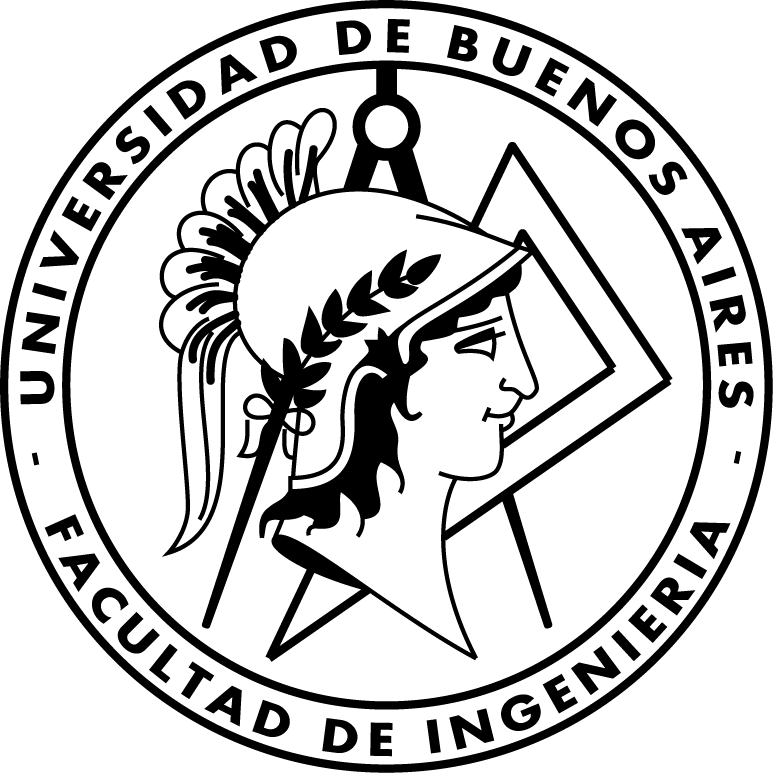
\includegraphics[width=6cm]{logofiuba.jpg}
    \centering
    \vfill
    \Huge \textbf{Trabajo Práctico 2 — Java}
    \vskip2cm
    \Large [7507/9502] Algoritmos y Programación III\\
    Grupo G15 \\
    Primer cuatrimestre 2022 \\
    \vfill
    Integrantes \\
    .\\
    \begin{tabular}{ | l | l | l | } % Datos del alumno
      \hline
      Alumno & Padrón & Email \\ \hline
      Alvaro Martín & 105040 & alvaro.martin1307@gmail.com \\ \hline
      Franco Macke & 105974 & fmacke@fi.uba.ar \\ \hline
      Guillermina Hoffmann & 104406 & ghoffmann@fi.uba.ar \\ \hline
      Juan Martin Iglesias & 107018 & jmiglesias@fi.uba.ar \\ \hline
  	\end{tabular}
    \vfill
    \vfill
\end{titlepage}

\tableofcontents % Índice general
\newpage

\section{Introducción}\label{sec:intro}

Es un juego programado en Java utilizado el paradigma orientado a objetos. Sumado a esto, se utilizaron las prácticas de Test Driven Development.

El concepto del juego es, utilizando un vehículo, atravesar una ciudad con obstáculos y llegar hasta una meta.

\section{Supuestos}\label{sec:supuestos}
  \begin{itemize}
    \item Una calle tiene solo un modificador.
    \item Se le debe indicar al vehiculo donde inicia.
    \item Se le debe indicar al vehiculo donde termina.
    \item Asumimos que solo hay un vehiculo.
    \item Las calles conectan 2 celdas.
    \item El tablero es de dimensión variable.
    \item Las sorpresas quedan en el tablero cuando se las cruza.
  \end{itemize}
\section{Diagramas de clase}\label{sec:diagramasdeclase}

A continuación se desarrollan los diagramas de clase que están presente en el modelo del juego. Más adelante, hay un esquema de secuencia donde se puede ver como interactuan entre si los objetos.

\begin{figure}[H]
  \centering
  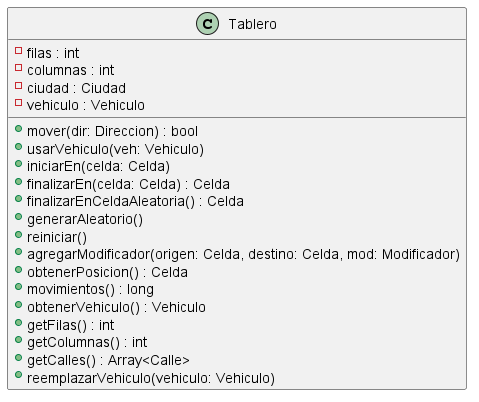
\includegraphics[width=1\textwidth]{diagramas/modelo-actual.png}
  \caption{\label{fig:seq01} Diagrama de clase Tablero}
\end{figure}

\begin{figure}[H]
  \centering
  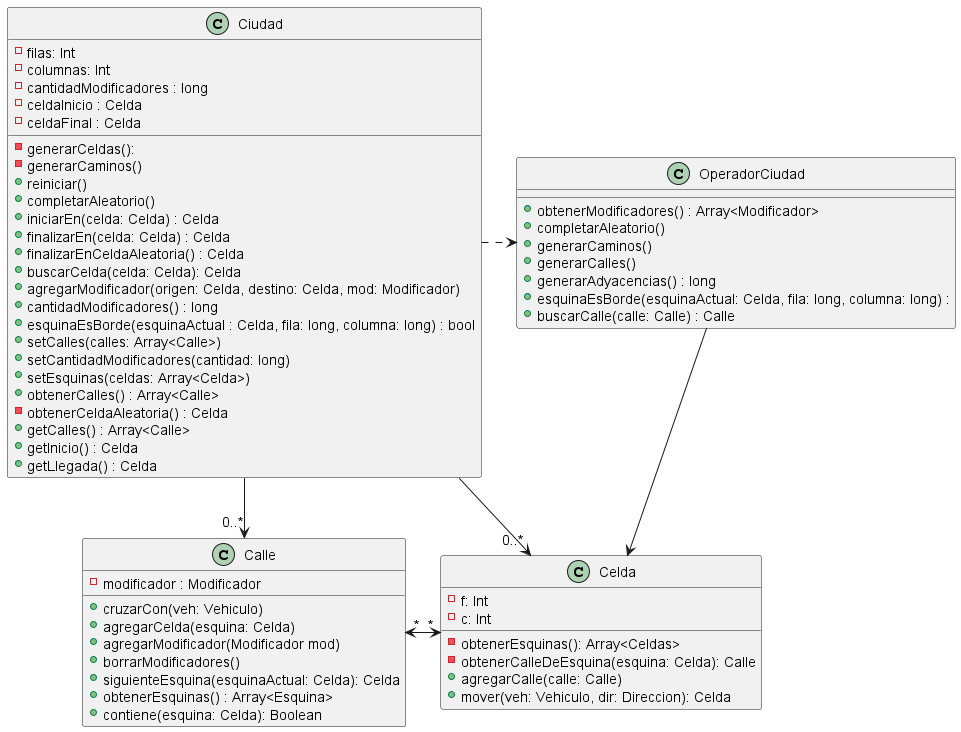
\includegraphics[width=1\textwidth]{diagramas/diagrama-ciudad.png}
  \caption{\label{fig:seq02} Diagrama de clase Ciudad}
\end{figure}


\begin{figure}[H]
  \centering
  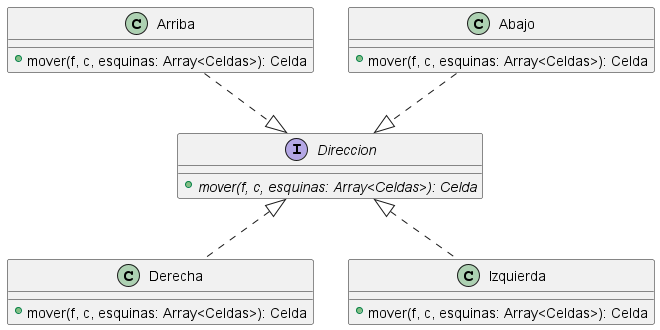
\includegraphics[width=1\textwidth]{diagramas/interface-direccion.png}
  \caption{\label{fig:seq03} Diagrama de clase Direccion}
\end{figure}

\begin{figure}[H]
  \centering
  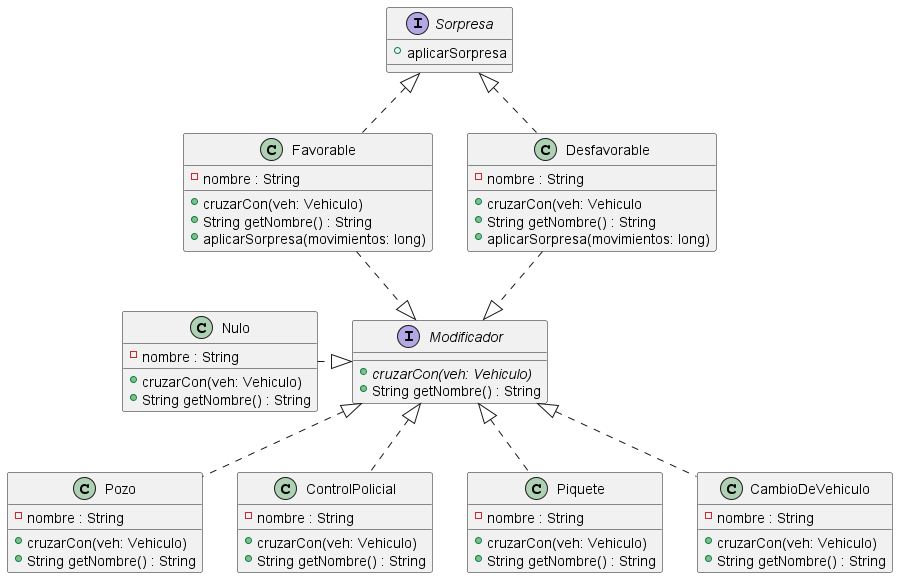
\includegraphics[width=1\textwidth]{diagramas/interface-modificador-sorpresa.png}
  \caption{\label{fig:seq04} Diagrama de clase Modificador}
\end{figure}

\begin{figure}[H]
  \centering
  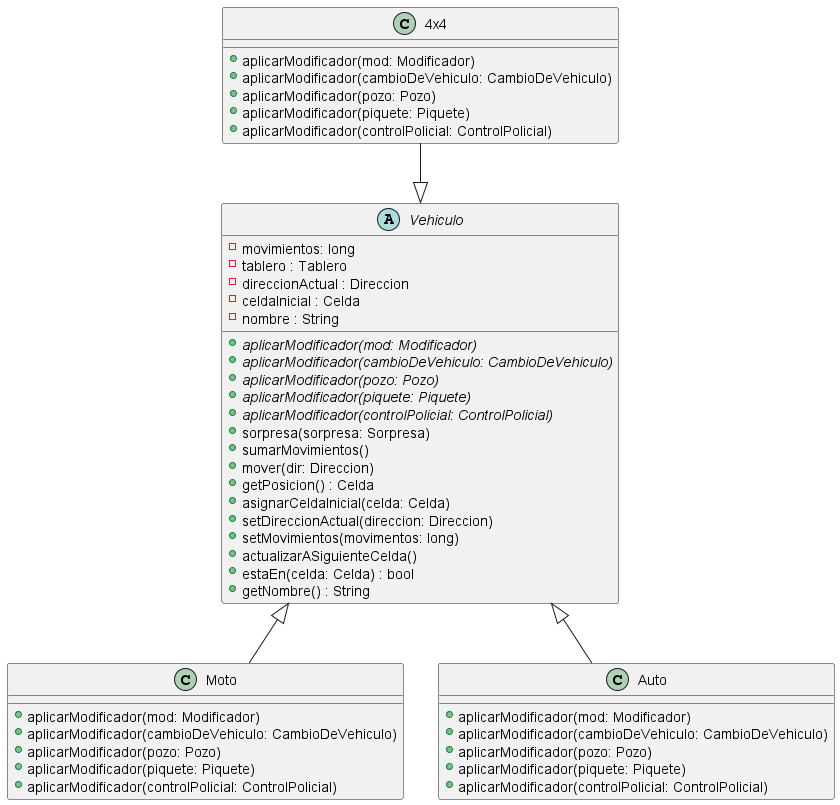
\includegraphics[width=1\textwidth]{diagramas/interface-vehiculo.png}
  \caption{\label{fig:seq05} Diagrama de clase Vehículo}
\end{figure}


\section{Detalles de implementación}\label{sec:implementacion}

En todas las clases se utilizaron los pilares de la programación orientada a objetos. Cada clase tiene su delegación correspondiente.

\subsubsection[Tablero]{Tablero}

La clase Tablero se encarga del manejo del juego. Delega su comportamiento a las clases correspondientes para el desarrollo.

\subsubsection[Ciudad]{Ciudad}

La clase Ciudad se encarga de la generación de la ciudad y el posicionamiento de los objetos del tablero.

\subsubsection[Modificador]{Modificador}

Esta interfaz está formada por el método “cruzarCon(Vehiculo vehiculo)”. Este método es utilizado por una instancia de la clase Calle para comunicarse con una clase que implementa Modificador.
Las clases que implementan esta interfaz son: Piquete, Favorable, Desfavorable, Nulo, Pozo, ControlPolicial y CambioDeVehiculo. En cada una de estas clases se implementa el método de la siguiente forma:

\begin{itemize}
  \item Nulo: Utiliza la instancia de vehiculo que recibe por argumento y llama al método “actualizarASiguienteCelda();”. Al cruzarse un Vehiculo con un Modificador Nulo solo cambia de celda. El modificador Nulo delega en el objeto Vehiculo el cambio de celda y suma de movimiento.
  \item En el caso de los modificadores Pozo, Piquete, ControlPolicial y CambioDeVehiculo todos estos utilizan la instancia de vehiculo que reciben por argumento y llaman al método “aplicarModificador(this);” enviando en cada caso una instancia de Modificador correspondiente a su tipo. Estos modificadores delegan en el Vehiculo aplicar el modificador ya que dependiendo del tipo de Vehiculo y tipo de Modificador se realizan diferentes acciones.
  \item En el caso de los modificadores Favorable y Desfavorable utilizan la instancia de vehiculo que reciben por argumento y llaman al método "sorpresa(this);", enviando por argumento una instancia de su tipo.
\end{itemize}
\subsubsection[Sorpresa]{Sorpresa}

Esta interfaz esta formada por el metodo  “long aplicarSorpresa(long movimientos);”  y es implementada por las clases Favorable y Desfavorable.
En este metodo se recibe la cantidad de movimientos del vehiculo y se calcula la penalizacion de movimientos. En el caso de Favorable se reduce la cantidad de movimientos en un 20\% y Desfavorable aumenta la cantidad de movimientos en un 25\%.

\subsubsection[Vehiculo]{Vehiculo}

Responde cuando el Tablero le manda el mensaje de mover con una dirección dada. A su vez, le envía un mensaje a su posición de mover y se va actualizar la posición a la correspondiente. Al aplicarse un Modificador al vehiculo, sabe como responder al mensaje que se le envía.


\subsubsection[Calle]{Calle}

La clase Calle guarda las referencias de 2 celdas, generando una conexión entre ellas. Cuando el vehiculo cruza por la calle, Calle le envía el mensaje al Modificador que se va a cruzar con un Vehículo.


\section{Excepciones}\label{sec:excepciones}
% Explicación de cada una de las excepciones creadas y con qué fin fueron creadas.

\begin{description}
\item[Exception] CeldaFueraDeRango: Se lanza cuando se quiere acceder a una celda que no existe dentro del tablero.
\end{description}

\section{Diagramas de secuencia}\label{sec:diagramasdesecuencia}
% Mostrar las secuencias interesantes que hayan implementado. Pueden agregar texto para explicar si algo no queda claro.

A continuación desarrollaremos el proceso del juego mediante los diagramas de secuencia.


\subsubsection[Una moto atraviesa la ciudad y se encuentra con un Pozo. Es penalizada en tres movimientos]{Una moto atraviesa la ciudad y se encuentra con un Pozo. Es penalizada en tres movimientos}

\begin{figure}[H]
  \centering
  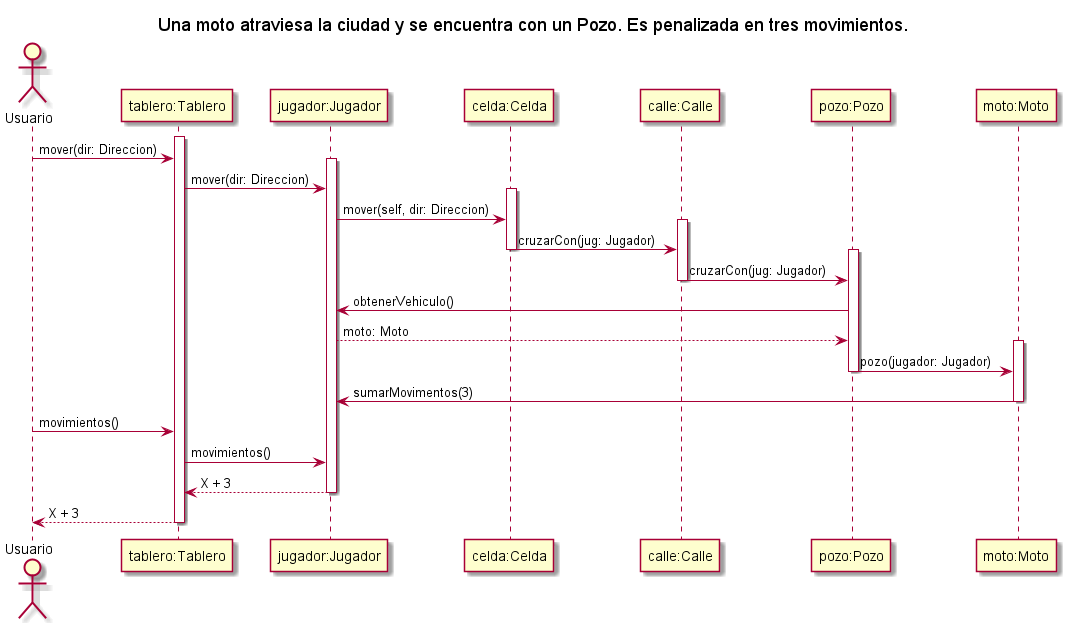
\includegraphics[width=1\textwidth]{diagramas/SecuenciaUnaMotoCruzaUnPozoYEsPenalizado.png}
  \caption{\label{fig:class01}Describe el caso donde una moto se cruza un pozo y recibe una penalización de 3 movimientos}
\end{figure}

\subsubsection[Un auto atraviesa la ciudad y se encuentra con un Pozo. Es penalizada en tres movimientos]{Un auto atraviesa la ciudad y se encuentra con un Pozo. Es penalizada en tres movimientos}

\begin{figure}[H]
  \centering
  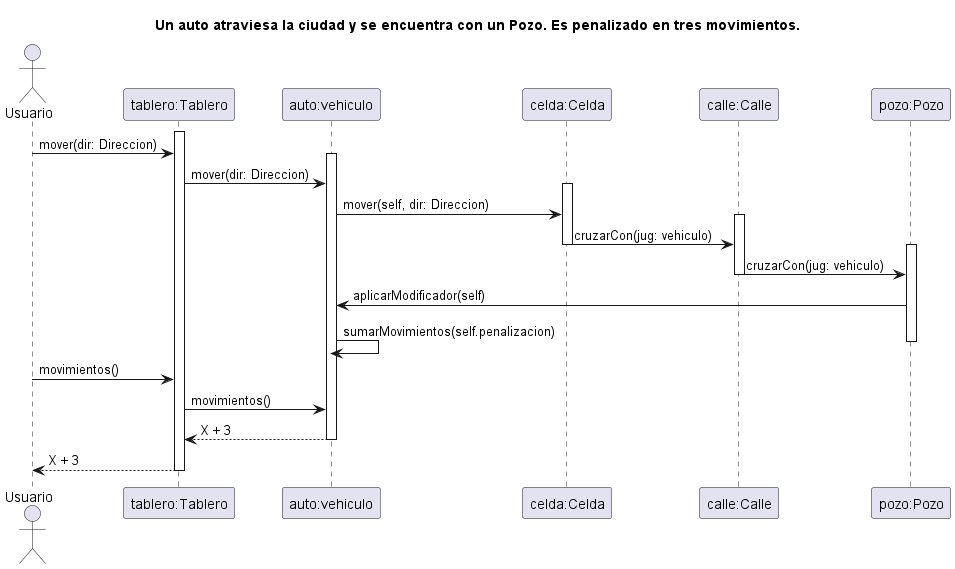
\includegraphics[width=1\textwidth]{diagramas/SecuenciaAutoCruzaUnPozoYEsPenalizado.png}
  \caption{\label{fig:class01} Describe el caso donde un auto atraviesa la ciudad y se encuentra un pozo, recibiendo una penalización de 3 movimientos}
\end{figure}


\subsubsection[Una 4x4 atraviesa la ciudad y se encuentra con un Pozo. No es penalizada]{Una 4x4 atraviesa la ciudad y se encuentra con un Pozo. No es penalizada}

\begin{figure}[H]
  \centering
  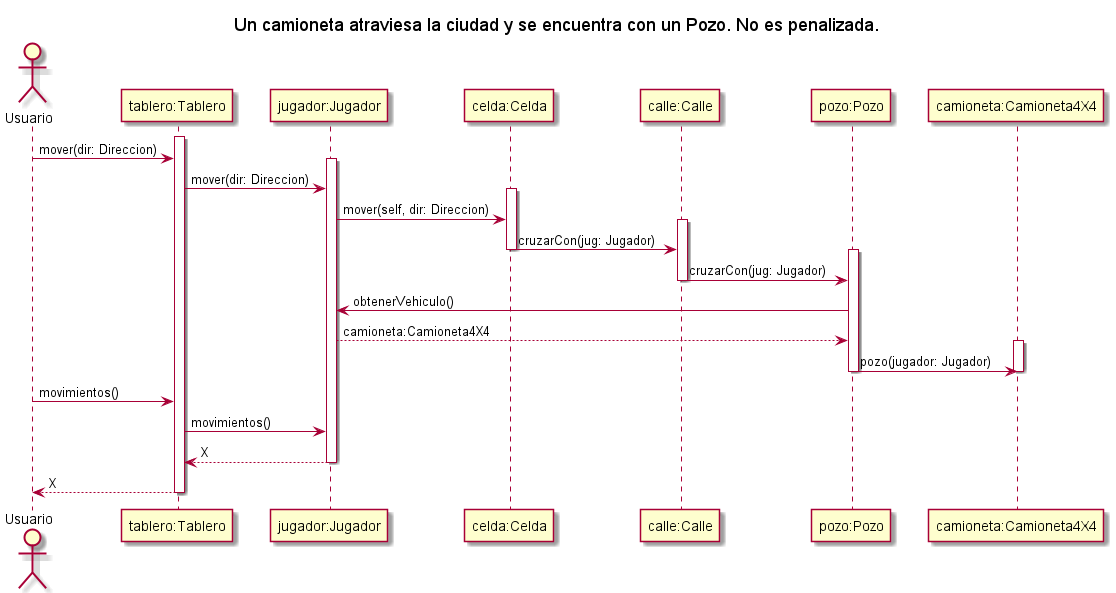
\includegraphics[width=1\textwidth]{diagramas/SecuenciaUnaCamionetaCruzaUnPozoYNoEsPenalizado.png}
  \caption{\label{fig:class01} Acá se ve el caso donde una camioneta se cruza con un pozo. No se ve afectado la cantidad de movimientos}
\end{figure}



\subsubsection[Un auto cambia de vehiculo]{Un auto cambia de vehiculo}

\begin{figure}[H]
  \centering
  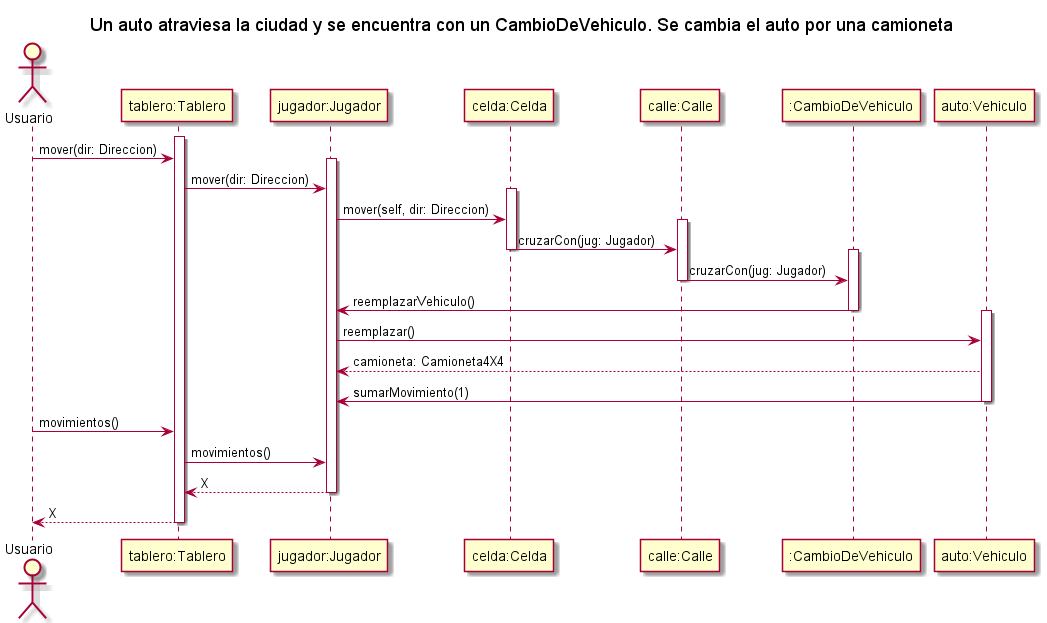
\includegraphics[width=1\textwidth]{diagramas/SecuenciaAutoCambiaVehiculo.png}
  \caption{\label{fig:class01} Cambio de vehículo de Auto a Camioneta}
\end{figure}



\subsubsection[Una moto cambia de vehiculo]{Una moto cambia de vehiculo}

\begin{figure}[H]
  \centering
  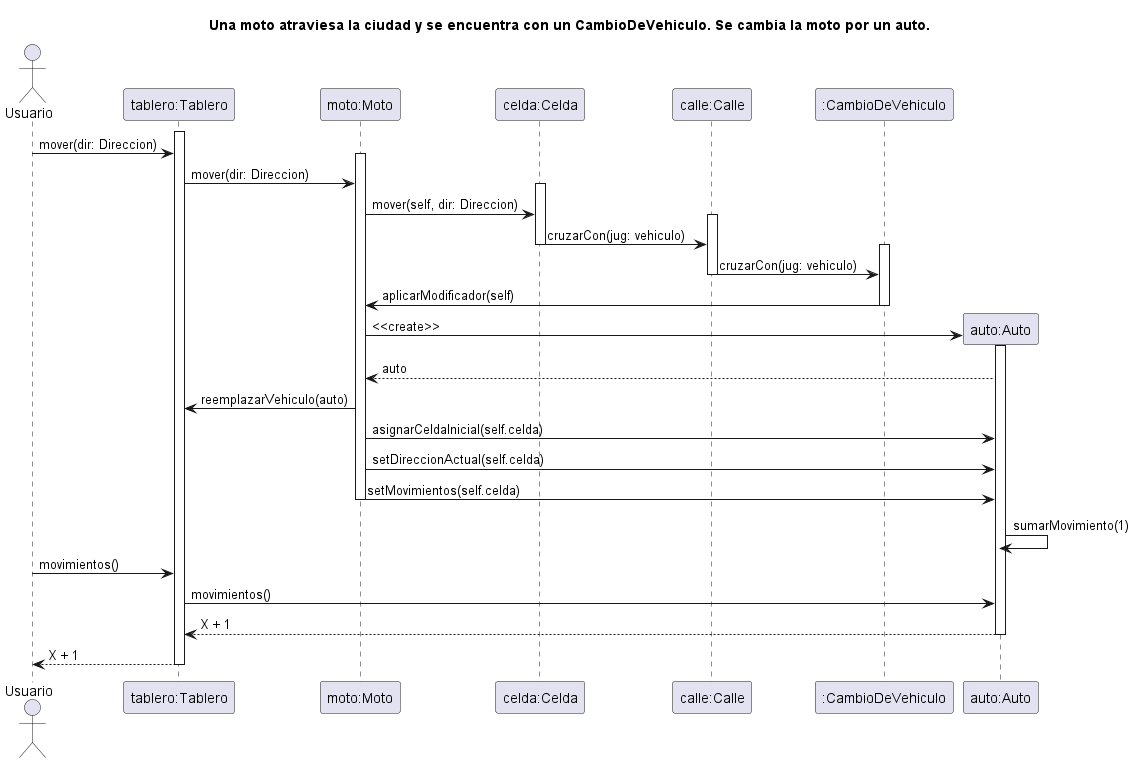
\includegraphics[width=1\textwidth]{diagramas/SecuenciaMotoCambiaVehiculo.png}
  \caption{\label{fig:class01}Cambio de vehículo de Moto a Auto}
\end{figure}

\subsubsection[Un Vehiculo se cruza con sorpresa Favorable]{Un Vehiculo se cruza con sorpresa Favorable}

\begin{figure}[H]
  \centering
  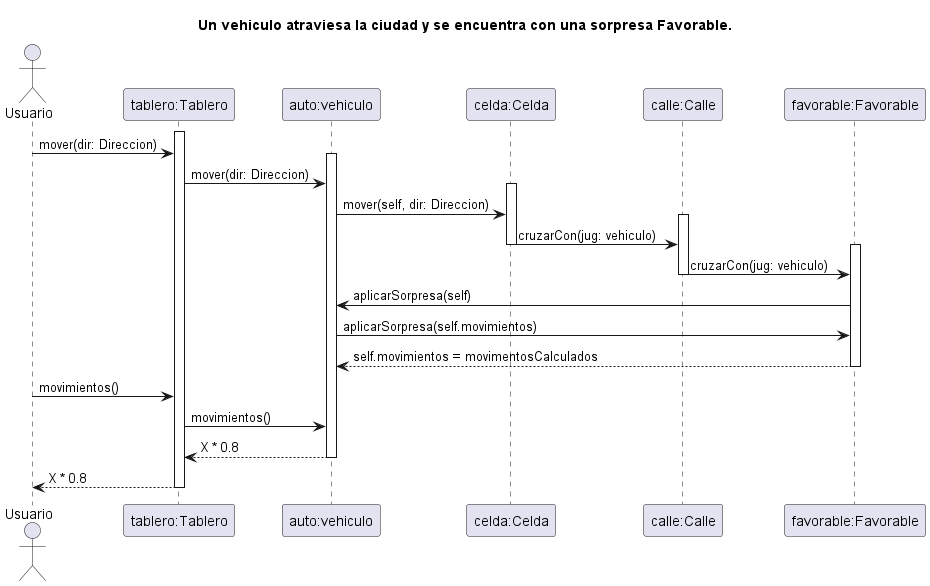
\includegraphics[width=1\textwidth]{diagramas/SecuenciaVehiculoCruzaSorpresaFavorable.png}
  \caption{\label{fig:class01}Un Vehiculo se cruza con sorpresa Favorable y se le restan movimientos.}
\end{figure}

\subsubsection[Un Vehiculo se cruza con sorpresa Desfavorable]{Un Vehiculo se cruza con sorpresa Desfavorable}

\begin{figure}[H]
  \centering
  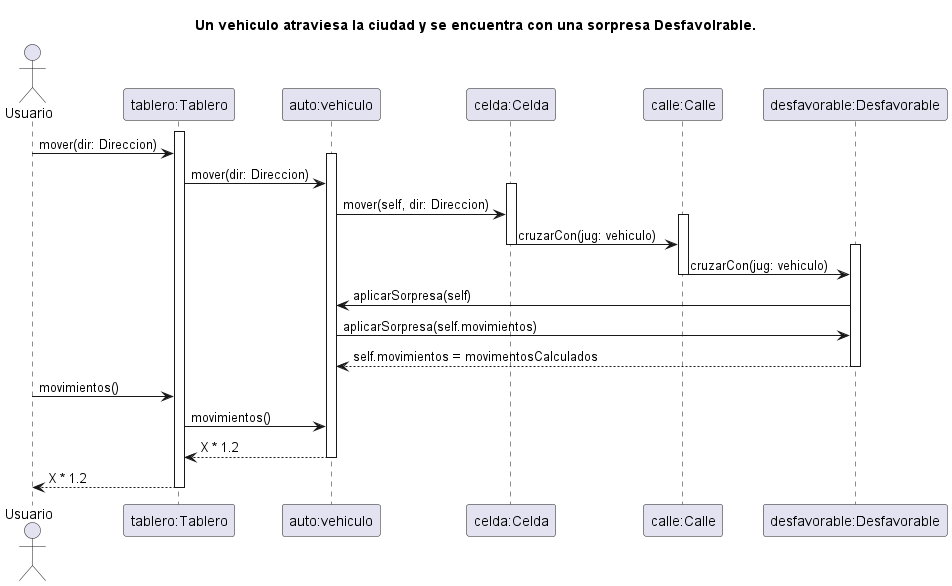
\includegraphics[width=1\textwidth]{diagramas/SecuenciaVehiculoCruzaSorpresaDesfavorable.png}
  \caption{\label{fig:class01}Un Vehiculo se cruza con sorpresa Desfavorable y se le suman movimientos.}
\end{figure}




\end{document}
